\documentclass[11pt,a4paper]{article}

\usepackage[top=20mm,bottom=26mm,left=20mm,right=20mm,headheight=15pt,footskip=12mm]{geometry}

\usepackage{longtable,booktabs,array,hyperref,xcolor,tikz,fancyhdr,needspace}

\usepackage{fontspec,xeCJK}

\setmainfont[Ligatures=TeXOff]{Times New Roman}

\setsansfont[Ligatures=TeXOff]{Times New Roman}

\setmonofont[Ligatures=TeXOff,WordSpace={1,1,1}]{Times New Roman}

\setCJKmainfont{Noto Serif CJK SC}

\setCJKsansfont{Noto Serif CJK SC}

\setCJKmonofont{Noto Serif CJK SC}

\newfontfamily\vulcanmathsymbols{Noto Serif CJK SC}

\XeTeXgenerateactualtext=1

\definecolor{vulcan}{HTML}{BB3E23}

\definecolor{vulcanblue}{HTML}{1B4F72}

\renewcommand{\thesection}{\Roman{section}}

\renewcommand{\thesubsection}{\Alph{subsection}}

\pgfdeclarelayer{connections}\pgfdeclarelayer{edge labels}\pgfsetlayers{connections,main,edge labels}

\hypersetup{hidelinks}

\newcolumntype{L}[1]{>{\raggedright\arraybackslash\hspace{0pt}}p{#1}}

\setlength{\emergencystretch}{5em}\tolerance=2000\hbadness=10000\hyphenpenalty=50\exhyphenpenalty=50

\setlength{\parindent}{0pt}\setlength{\parskip}{5pt}

\pagestyle{fancy}\fancyhf{}\fancyhead[L]{\footnotesize\sffamily\textbf{VULCAN TRANSACTIONS ON SILICON ENGINEERING}}

\fancyhead[R]{\footnotesize\sffamily RTL Microarchitecture \& Silicon Signoff}\fancyfoot[C]{\footnotesize\sffamily Page \thepage}

\begin{document}

{\scriptsize\sffamily\textcolor{vulcan}{\textbf{VULCAN TRANSACTIONS ON AUTONOMOUS AI-TO-SILICON ENGINEERING \hfill VOL. 2026 \textperiodcentered{} ARCHITECTURAL SIGNOFF PAPER}}\par}

\vspace{1pt}\textcolor{vulcan}{\rule{\textwidth}{1.2pt}}\vspace{4pt}

\begin{center}

{\sffamily\LARGE\bfseries BILLET-T1: Parameterized Fixed-Point Complex FFT RTL IP\par}\vspace{3pt}

{\small\sffamily\textbf{Sufeng Guo (\allowbreak{}sufeng\_\allowbreak{}guo@smail.nju.edu.cn)\allowbreak{}} \textperiodcentered{} Microsoft Research Asia \textperiodcentered{} Technical Design and Verification Report\par}\vspace{1pt}

{\scriptsize\sffamily\textcolor{black!75}{Silicon Platform: Intel Arria 10 GX (\texttt{10AX115N3F40E2SG}) PCIe Gen3x8 \textperiodcentered{} Toolchain: Icarus Verilog 12.0 / Yosys 0.33 / Quartus Prime 17.1 STA \textperiodcentered{} 24 October 2026 (\allowbreak{}2026-10-24 20:12 UTC+\allowbreak{}8 Beijing Time)\allowbreak{}}\par}

\end{center}\vspace{2pt}

\renewcommand{\abstractname}{\textcolor{vulcanblue}{Abstract}}\begin{abstract}\noindent BILLET-T1 implements a forward complex radix-2 FFT with signed 16-bit Q1.15 input and output,\allowbreak{} natural-order streaming interfaces,\allowbreak{} deterministic floor quantization and nominal 1/\allowbreak{}N normalization. The default transform length is 256; supported lengths are powers of two from 2 through 256. The delivered product is technology-independent RTL IP for integration into a larger digital system,\allowbreak{} not a fabricated or physically signed-off chip. A single reused butterfly operates on two ping-pong sample banks under an explicit synchronous READ/\allowbreak{}WRITE schedule. Independent verification at N=\allowbreak{}2,\allowbreak{}16,\allowbreak{}64,\allowbreak{}256 compared 9,\allowbreak{}454 accepted complex outputs against a separately authored integer oracle with zero scalar mismatches. Every designated rail-safe quality frame met cosine similarity >=\allowbreak{}0.999 and SQNR >=\allowbreak{}30 dB against a direct floating-point DFT. Four functional mutations were detected,\allowbreak{} and generic synthesis reported zero latches at all four required sizes. These results are supported by E014–E016.\par\vspace{2pt}{\scriptsize\textbf{\textcolor{vulcanblue}{Index Terms---}}Autonomous RTL Generation, SystemVerilog, Intel Arria 10 GX FPGA, TimeQuest 100~MHz+ Timing Closure, PCIe Gen3x8 Hardware-in-the-Loop (HIL), Bit-Exact Fixed-Point Verification.}\end{abstract}\vspace{2pt}

\needspace{5\baselineskip}\section{Architecture and design rationale}

The architecture favors explicit memory ownership and deterministic timing over overlapping frames or maximum throughput. Natural-order inputs are stored at bit-reversed addresses in bank 0. Each decimation-in-time stage reads two operands from one bank and writes two results to the other on the following edge. Bank ownership changes only after the stage finishes. One combinational butterfly supplies four signed real multiplications,\allowbreak{} widened additions,\allowbreak{} unconditional stage scaling and final component clamps. The top literally instantiates the scheduler,\allowbreak{} bit-reversal unit,\allowbreak{} twiddle ROM and butterfly; the package supplies shared numerical constants. The two sample banks contain 64*\allowbreak{}N bits in total,\allowbreak{} or 16,\allowbreak{}384 bits at N=\allowbreak{}256,\allowbreak{} excluding holding registers. Their logical two-port organization does not imply a particular SRAM macro mapping. E001–E008 describe and implement these responsibilities.

\begin{center}\begin{minipage}{\textwidth}\centering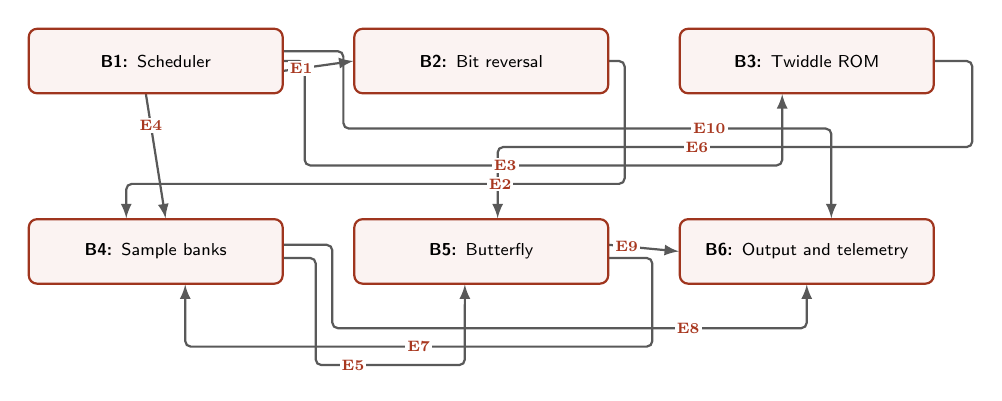
\begin{tikzpicture}[scale=0.78,transform shape,every node/.style={font=\footnotesize\sffamily},>=latex]

\node[draw=vulcan!85!black,thick,rounded corners=3pt,fill=vulcan!6,text width=3.9cm,minimum height=1.05cm,align=center] (b0) at (0.0,0.0) {\textbf{B1:} Scheduler};

\node[draw=vulcan!85!black,thick,rounded corners=3pt,fill=vulcan!6,text width=3.9cm,minimum height=1.05cm,align=center] (b1) at (5.3,0.0) {\textbf{B2:} Bit reversal};

\node[draw=vulcan!85!black,thick,rounded corners=3pt,fill=vulcan!6,text width=3.9cm,minimum height=1.05cm,align=center] (b2) at (10.6,0.0) {\textbf{B3:} Twiddle ROM};

\node[draw=vulcan!85!black,thick,rounded corners=3pt,fill=vulcan!6,text width=3.9cm,minimum height=1.05cm,align=center] (b3) at (0.0,-3.1) {\textbf{B4:} Sample banks};

\node[draw=vulcan!85!black,thick,rounded corners=3pt,fill=vulcan!6,text width=3.9cm,minimum height=1.05cm,align=center] (b4) at (5.3,-3.1) {\textbf{B5:} Butterfly};

\node[draw=vulcan!85!black,thick,rounded corners=3pt,fill=vulcan!6,text width=3.9cm,minimum height=1.05cm,align=center] (b5) at (10.6,-3.1) {\textbf{B6:} Output and telemetry};

\begin{pgfonlayer}{connections}

\draw[->,thick,black!65] ([yshift=-0.160cm]b0.east) -- coordinate[pos=0.25] (e0) ([yshift=0.000cm]b1.west);

\draw[->,thick,black!65,rounded corners=2pt] ([yshift=0.000cm]b1.east) -- (7.635,0.000) -- (7.635,-2.000) -- coordinate[pos=0.25] (e1) (-0.480,-2.000) -- ([xshift=-0.480cm]b3.north);

\draw[->,thick,black!65,rounded corners=2pt] ([yshift=0.000cm]b0.east) -- (2.425,0.000) -- (2.425,-1.700) -- coordinate[pos=0.42] (e2) (10.200,-1.700) -- ([xshift=-0.400cm]b2.south);

\draw[->,thick,black!65] ([xshift=-0.160cm]b0.south) -- coordinate[pos=0.25] (e3) ([xshift=0.160cm]b3.north);

\draw[->,thick,black!65,rounded corners=2pt] ([yshift=-0.107cm]b3.east) -- (2.605,-3.207) -- (2.605,-4.950) -- coordinate[pos=0.25] (e4) (5.033,-4.950) -- ([xshift=-0.267cm]b4.south);

\draw[->,thick,black!65,rounded corners=2pt] ([yshift=0.000cm]b2.east) -- (13.295,0.000) -- (13.295,-1.400) -- coordinate[pos=0.58] (e5) (5.567,-1.400) -- ([xshift=0.267cm]b4.north);

\draw[->,thick,black!65,rounded corners=2pt] ([yshift=-0.107cm]b4.east) -- (8.085,-3.207) -- (8.085,-4.650) -- coordinate[pos=0.50] (e6) (0.480,-4.650) -- ([xshift=0.480cm]b3.south);

\draw[->,thick,black!65,rounded corners=2pt] ([yshift=0.107cm]b3.east) -- (2.875,-2.993) -- (2.875,-4.350) -- coordinate[pos=0.75] (e7) (10.600,-4.350) -- ([xshift=0.000cm]b5.south);

\draw[->,thick,black!65] ([yshift=0.107cm]b4.east) -- coordinate[pos=0.25] (e8) ([yshift=0.000cm]b5.west);

\draw[->,thick,black!65,rounded corners=2pt] ([yshift=0.160cm]b0.east) -- (3.055,0.160) -- (3.055,-1.100) -- coordinate[pos=0.75] (e9) (11.000,-1.100) -- ([xshift=0.400cm]b5.north);

\end{pgfonlayer}

\begin{pgfonlayer}{edge labels}

\node[fill=white,inner sep=1pt,font=\scriptsize\bfseries,text=vulcan!90!black] at (e0) {E1};

\node[fill=white,inner sep=1pt,font=\scriptsize\bfseries,text=vulcan!90!black] at (e1) {E2};

\node[fill=white,inner sep=1pt,font=\scriptsize\bfseries,text=vulcan!90!black] at (e2) {E3};

\node[fill=white,inner sep=1pt,font=\scriptsize\bfseries,text=vulcan!90!black] at (e3) {E4};

\node[fill=white,inner sep=1pt,font=\scriptsize\bfseries,text=vulcan!90!black] at (e4) {E5};

\node[fill=white,inner sep=1pt,font=\scriptsize\bfseries,text=vulcan!90!black] at (e5) {E6};

\node[fill=white,inner sep=1pt,font=\scriptsize\bfseries,text=vulcan!90!black] at (e6) {E7};

\node[fill=white,inner sep=1pt,font=\scriptsize\bfseries,text=vulcan!90!black] at (e7) {E8};

\node[fill=white,inner sep=1pt,font=\scriptsize\bfseries,text=vulcan!90!black] at (e8) {E9};

\node[fill=white,inner sep=1pt,font=\scriptsize\bfseries,text=vulcan!90!black] at (e9) {E10};

\end{pgfonlayer}

\end{tikzpicture}\par\vspace{3pt}

{\small\textbf{Figure 1:} Top-level microarchitectural functional block map and directed inter-module bus topology.}\end{minipage}\end{center}

{\small\renewcommand{\arraystretch}{1.18}\begin{longtable}{@{}L{0.24\textwidth}|L{0.7\textwidth}@{}}\toprule

\textbf{Block} & \textbf{Responsibility}\\\midrule\endhead

B1: Scheduler & billet\_\allowbreak{}t1\_\allowbreak{}buffer\_\allowbreak{}sched sequences LOAD,\allowbreak{} READ,\allowbreak{} WRITE,\allowbreak{} FETCH and SEND; counts accepted samples; generates stage addresses; controls bank ownership; and implements output handshaking and completion.\\[2pt]\hline

B2: Bit reversal & billet\_\allowbreak{}t1\_\allowbreak{}bitrev reverses exactly LOG2\_\allowbreak{}N bits of the natural load index,\allowbreak{} placing accepted inputs in the order required by the iterative decimation-in-time transform.\\[2pt]\hline

B3: Twiddle ROM & billet\_\allowbreak{}t1\_\allowbreak{}twiddle\_\allowbreak{}rom supplies literal signed Q1.15 forward-transform coefficients. Smaller transforms select a stride through the exact 256-point half-circle table.\\[2pt]\hline

B4: Sample banks & Two N-deep banks in billet\_\allowbreak{}t1\_\allowbreak{}top store packed 32-bit complex samples. Synchronous reads capture operand pairs; alternate-bank writes commit butterfly results without read-during-write dependence.\\[2pt]\hline

B5: Butterfly & billet\_\allowbreak{}t1\_\allowbreak{}butterfly calculates the complex product,\allowbreak{} floor quantization,\allowbreak{} divide-by-two scaling and four signed clamps. Its sat\_\allowbreak{}inc output reports scalar clamp events.\\[2pt]\hline

B6: Output and telemetry & Top-level logic reuses the port-A operand register as the output holding register,\allowbreak{} masks invalid payloads to zero,\allowbreak{} and maintains reset-cleared sticky saturation telemetry.\\[2pt]\hline

\bottomrule\end{longtable}}

{\small\renewcommand{\arraystretch}{1.18}\begin{longtable}{@{}L{0.24\textwidth}|L{0.7\textwidth}@{}}\toprule

\textbf{Directed relationship} & \textbf{Meaning}\\\midrule\endhead

E1: B1 to B2 & Natural load index\\[2pt]\hline

E2: B2 to B4 & Bit-reversed load address\\[2pt]\hline

E3: B1 to B3 & Stage coefficient address\\[2pt]\hline

E4: B1 to B4 & Bank selection,\allowbreak{} addresses and phase enables\\[2pt]\hline

E5: B4 to B5 & Registered source operands\\[2pt]\hline

E6: B3 to B5 & Complex coefficient\\[2pt]\hline

E7: B5 to B4 & Two destination results on WRITE\\[2pt]\hline

E8: B4 to B6 & Final-bank output fetch\\[2pt]\hline

E9: B5 to B6 & Clamp increment,\allowbreak{} accumulated only on WRITE\\[2pt]\hline

E10: B1 to B6 & Output validity,\allowbreak{} bin index and completion\\[2pt]\hline

\bottomrule\end{longtable}}

\needspace{9\baselineskip}\section{Interfaces and configuration}

{\small\renewcommand{\arraystretch}{1.18}\begin{longtable}{@{}L{0.21\textwidth}|L{0.12\textwidth}|L{0.12\textwidth}|L{0.45\textwidth}@{}}\toprule

\textbf{Signal /\allowbreak{} group} & \textbf{Direction} & \textbf{Width} & \textbf{Contract}\\\midrule\endhead

clk,\allowbreak{} rst\_\allowbreak{}n & Input & 1 bit each & Single clock and asynchronous active-low reset. Reset overrides transfers,\allowbreak{} aborts the current transaction and forces every public output to zero. Sample memories are not reset.\\[2pt]\hline

in\_\allowbreak{}valid,\allowbreak{} in\_\allowbreak{}ready & Input /\allowbreak{} output & 1 bit each & A sample is accepted on a rising edge only when both are high before the edge. in\_\allowbreak{}ready is asserted in LOAD after reset release and deasserted throughout computation and output.\\[2pt]\hline

in\_\allowbreak{}re,\allowbreak{} in\_\allowbreak{}im,\allowbreak{} in\_\allowbreak{}last & Input & Two signed 16-bit components; 1-bit marker & Natural-order Q1.15 samples. Exactly N\_\allowbreak{}POINTS accepted beats define a frame. in\_\allowbreak{}last is advisory and has no state or datapath effect; early or absent markers do not alter framing.\\[2pt]\hline

out\_\allowbreak{}valid,\allowbreak{} out\_\allowbreak{}ready & Output /\allowbreak{} input & 1 bit each & An output is consumed only on a rising-edge valid/\allowbreak{}ready handshake. While valid is high and ready is low,\allowbreak{} payload,\allowbreak{} bin index and last remain stable.\\[2pt]\hline

out\_\allowbreak{}re,\allowbreak{} out\_\allowbreak{}im & Output & Two signed 16-bit components & Q1.15 frequency-domain results with nominal 1/\allowbreak{}N scaling. Both components are zero whenever out\_\allowbreak{}valid is zero.\\[2pt]\hline

out\_\allowbreak{}bin\_\allowbreak{}idx,\allowbreak{} out\_\allowbreak{}last & Output & A bits; 1 bit & Natural bin index 0 through N\_\allowbreak{}POINTS-1. out\_\allowbreak{}last accompanies only the valid final bin. Both outputs are zero outside valid output cycles.\\[2pt]\hline

frame\_\allowbreak{}done & Output & 1 bit & One-cycle pulse immediately after the edge accepting the final output. in\_\allowbreak{}ready is simultaneously restored; the next frame can begin on the following edge.\\[2pt]\hline

saturation\_\allowbreak{}count,\allowbreak{} overflow\_\allowbreak{}flag & Output & Unsigned 32 bits; 1 bit & Sticky scalar clamp count and sticky indication of any clamp. Count increments by 0..4 per committed butterfly and saturates at 0xffffff\allowbreak{}ff. Both clear only on reset.\\[2pt]\hline

\bottomrule\end{longtable}}

{\small\renewcommand{\arraystretch}{1.18}\begin{longtable}{@{}L{0.22\textwidth}|L{0.21\textwidth}|L{0.49\textwidth}@{}}\toprule

\textbf{Parameter} & \textbf{Default} & \textbf{Meaning /\allowbreak{} supported values}\\\midrule\endhead

N\_\allowbreak{}POINTS & 256 & Legal values are 2,\allowbreak{}4,\allowbreak{}8,\allowbreak{}16,\allowbreak{}32,\allowbreak{}64,\allowbreak{}128,\allowbreak{}256. Full transform behavior and synthesis were exercised at 2,\allowbreak{}16,\allowbreak{}64,\allowbreak{}256; coefficient and permutation units were exercised at every legal size.\\[2pt]\hline

LOG2\_\allowbreak{}N & \$clog2(\allowbreak{}N\_\allowbreak{}POINTS)\allowbreak{} for legal configurations & Derived stage count; must not be overridden inconsistently. The implementation uses a diagnostic-safe fallback of 1 when N\_\allowbreak{}POINTS<=\allowbreak{}1,\allowbreak{} without supporting those configurations.\\[2pt]\hline

Derived widths A and S & A=\allowbreak{}max(\allowbreak{}1,\allowbreak{}LOG2\_\allowbreak{}N)\allowbreak{}; S=\allowbreak{}max(\allowbreak{}1,\allowbreak{}\$clog2(\allowbreak{}LOG2\_\allowbreak{}N)\allowbreak{})\allowbreak{} & A sizes sample addresses and bin indices; S sizes stage indices. Minimum widths preserve the legal one-stage N=\allowbreak{}2 boundary. Invalid configurations select an inert branch with an explicit simulation parameter diagnostic.\\[2pt]\hline

\bottomrule\end{longtable}}

\needspace{16\baselineskip}\section{Behavior and corner cases}

\subsection{Coefficient and arithmetic contract}

Each code represents its signed integer value divided by 32768. For k=\allowbreak{}0..N/\allowbreak{}2-1,\allowbreak{} coefficient components are clamp16(\allowbreak{}round\_\allowbreak{}half\_\allowbreak{}away\_\allowbreak{}from\_\allowbreak{}zero(\allowbreak{}32768*\allowbreak{}cos(\allowbreak{}2*\allowbreak{}pi*\allowbreak{}k/\allowbreak{}N)\allowbreak{})\allowbreak{})\allowbreak{} and clamp16(\allowbreak{}round\_\allowbreak{}half\_\allowbreak{}away\_\allowbreak{}from\_\allowbreak{}zero(\allowbreak{}-32768*\allowbreak{}sin(\allowbreak{}2*\allowbreak{}pi*\allowbreak{}k/\allowbreak{}N)\allowbreak{})\allowbreak{})\allowbreak{}. Thus +\allowbreak{}1 maps to 32767 and -1 to -32768. Four exact 16x16-to-32-bit products form P\_\allowbreak{}re=\allowbreak{}B\_\allowbreak{}re*\allowbreak{}W\_\allowbreak{}re-B\_\allowbreak{}im*\allowbreak{}W\_\allowbreak{}im and P\_\allowbreak{}im=\allowbreak{}B\_\allowbreak{}re*\allowbreak{}W\_\allowbreak{}im+\allowbreak{}B\_\allowbreak{}im*\allowbreak{}W\_\allowbreak{}re after sign extension into 33 bits. For each component c,\allowbreak{} T\_\allowbreak{}c=\allowbreak{}floor(\allowbreak{}P\_\allowbreak{}c/\allowbreak{}32768)\allowbreak{},\allowbreak{} U\_\allowbreak{}c=\allowbreak{}floor(\allowbreak{}(\allowbreak{}A\_\allowbreak{}c+\allowbreak{}T\_\allowbreak{}c)\allowbreak{}/\allowbreak{}2)\allowbreak{},\allowbreak{} and V\_\allowbreak{}c=\allowbreak{}floor(\allowbreak{}(\allowbreak{}A\_\allowbreak{}c-T\_\allowbreak{}c)\allowbreak{}/\allowbreak{}2)\allowbreak{}. The latter sums use 34 bits. Only U and V are clamped to [\allowbreak{}-32768,\allowbreak{}32767]\allowbreak{}. Arithmetic shifts implement floor rounding,\allowbreak{} including for negative values; there is no rounding bias or premature narrowing. E002 and E005 define this exact contract.

\needspace{10\baselineskip}\subsection{Scaling and full-scale clipping}

Every stage unconditionally divides by two,\allowbreak{} producing nominal 1/\allowbreak{}N normalization. This does not guarantee zero clipping for independently full-scale real and imaginary components: complex rotation can move a square-domain input beyond a component rail. The documented N=\allowbreak{}16 counterexample produces A=\allowbreak{}(\allowbreak{}-32767,\allowbreak{}-32767)\allowbreak{},\allowbreak{} T=\allowbreak{}(\allowbreak{}-46339,\allowbreak{}0)\allowbreak{},\allowbreak{} and an unbounded real U=\allowbreak{}-39553,\allowbreak{} which correctly clamps to -32768. Widened arithmetic prevents unintended intermediate wraparound; telemetry reports intentional clamps. Rail-safe quality cases and deliberately clipped stress cases therefore have distinct floating-point expectations.

\needspace{10\baselineskip}\subsection{Conflict-free stage schedule}

For stage s,\allowbreak{} half=\allowbreak{}2\textasciicircum{}s,\allowbreak{} span=\allowbreak{}2\textasciicircum{}(\allowbreak{}s+\allowbreak{}1)\allowbreak{},\allowbreak{} a=\allowbreak{}base+\allowbreak{}j,\allowbreak{} b=\allowbreak{}a+\allowbreak{}half and k=\allowbreak{}j*\allowbreak{}N/\allowbreak{}span,\allowbreak{} with group bases separated by span and j=\allowbreak{}0..half-1. A READ edge captures both source operands; the following WRITE commits both results at distinct destination addresses. Addresses remain constant across the pair. Every address is covered once per stage,\allowbreak{} and the banks swap only after the final write. The final bank is LOG2\_\allowbreak{}N modulo 2. Scheduler outputs load\_\allowbreak{}we,\allowbreak{} stage\_\allowbreak{}read,\allowbreak{} stage\_\allowbreak{}write and output\_\allowbreak{}fetch identify impending edge operations; load\_\allowbreak{}addr is natural-order before the separate bit reversal. E001 and E004 document these internal integration semantics.

\needspace{10\baselineskip}\subsection{Exact edge latency}

Let F accept the final input and C=\allowbreak{}N*\allowbreak{}LOG2\_\allowbreak{}N. F+\allowbreak{}1 captures the first operand pair; F+\allowbreak{}2 commits its results; F+\allowbreak{}C commits the final butterfly. F+\allowbreak{}C+\allowbreak{}1 fetches bin 0 and makes out\_\allowbreak{}valid high after the edge; its earliest handshake is F+\allowbreak{}C+\allowbreak{}2. A nonfinal handshake at H clears valid,\allowbreak{} H+\allowbreak{}1 fetches the next bin,\allowbreak{} and H+\allowbreak{}2 is its earliest handshake. Without output stalls,\allowbreak{} final acceptance is D=\allowbreak{}F+\allowbreak{}C+\allowbreak{}2*\allowbreak{}N: 6,\allowbreak{}96,\allowbreak{}512,\allowbreak{}2560 edges after F for N=\allowbreak{}2,\allowbreak{}16,\allowbreak{}64,\allowbreak{}256 respectively. At N=\allowbreak{}256,\allowbreak{} computation consumes 2048 edges and output fetch/\allowbreak{}send consumes 512. These are clock counts,\allowbreak{} not measured time or frequency.

\needspace{10\baselineskip}\subsection{Framing,\allowbreak{} stalls and reset}

Input gaps are permitted,\allowbreak{} and subsequent frames may be continuously offered,\allowbreak{} but unaccepted input beats must remain stable. Frames are serialized without overlap. SEND performs no new fetch while stalled,\allowbreak{} so neither payload nor telemetry is repeatedly updated. Reset suppresses completion for aborted frames and clears holding registers and telemetry. A fresh complete frame initializes storage before any subsequent transform can expose data,\allowbreak{} preventing stale-frame leakage without resetting the banks.

\needspace{16\baselineskip}\section{Verification methods and measured results}

\subsection{Bit-exact FFT results and telemetry}

\textbf{Method.} Independent Python integer arithmetic reconstructed coefficients,\allowbreak{} stage scaling and clamp events. Icarus simulations exercised impulses,\allowbreak{} signed complex DC,\allowbreak{} nontrivial and near-Nyquist tones,\allowbreak{} multitone,\allowbreak{} seeded random,\allowbreak{} asymmetric,\allowbreak{} low-level and full-square inputs. The base seed was 2970740481; each size used base+\allowbreak{}N.

\textbf{Result.} N=\allowbreak{}2 completed 23 frames and 46 outputs; N=\allowbreak{}16,\allowbreak{}64,\allowbreak{}256 each completed 28 frames and respectively 448,\allowbreak{}1792,\allowbreak{}7168 outputs. Across 107 completed frames and 9,\allowbreak{}454 complex outputs,\allowbreak{} scalar mismatches were zero and telemetry matched independent clamp accounting.

{\small Evidence: E009,\allowbreak{} E014}

\needspace{12\baselineskip}\subsection{Per-frame numerical quality against an independent DFT}

\textbf{Method.} A separate O(\allowbreak{}N\textasciicircum{}2)\allowbreak{} floating-point forward DFT divided by N evaluated actual quantized inputs. Preselected amplitudes included impulse 30000+\allowbreak{}j12000,\allowbreak{} DC 12000+\allowbreak{}j7000,\allowbreak{} tone radius 20000,\allowbreak{} multitone radii 9000/\allowbreak{}6000/\allowbreak{}4000 and random components within [\allowbreak{}-16000,\allowbreak{}16000]\allowbreak{}. Real and imaginary components formed one comparison vector.

\textbf{Result.} Every designated quality frame at N=\allowbreak{}16,\allowbreak{}64,\allowbreak{}256 had zero clamps,\allowbreak{} cosine >=\allowbreak{}0.999 and SQNR >=\allowbreak{}30 dB. Representative bin-1 tones yielded SQNR 80.51/\allowbreak{}75.16/\allowbreak{}70.43 dB,\allowbreak{} cosine 0.999999997/\allowbreak{}0.999999990/\allowbreak{}0.999999967,\allowbreak{} maximum error 1.205/\allowbreak{}2.039/\allowbreak{}3.111 codes and RMSE 0.333/\allowbreak{}0.308/\allowbreak{}0.266 codes respectively. Complete per-frame metrics,\allowbreak{} including repeated reset-recovery frames,\allowbreak{} are retained in the behavior receipt.

{\small Evidence: E009,\allowbreak{} E014}

\needspace{12\baselineskip}\subsection{Truthful full-scale and low-level behavior}

\textbf{Method.} Full-square corner/\allowbreak{}random frames and a directed clipping counterexample retained integer exactness requirements while measuring floating error without imposing rail-safe quality thresholds.

\textbf{Result.} The 256-point directed counterexample produced exactly one clamp,\allowbreak{} SQNR 16.69 dB and cosine 0.996219. The low-level case measured SQNR -21.37 dB and cosine 0.138854,\allowbreak{} illustrating quantization-dominated behavior rather than a hidden pass. Zero-frame error was zero; undefined zero-vector cosine remained null.

{\small Evidence: E002,\allowbreak{} E014}

\needspace{12\baselineskip}\subsection{Streaming protocol,\allowbreak{} edge timing and memory scheduling}

\textbf{Method.} Cycle-by-cycle public-pin comparisons checked pre-edge handshakes and post-edge outputs under input gaps,\allowbreak{} continuous busy-period demand,\allowbreak{} early/\allowbreak{}missing last markers,\allowbreak{} long/\allowbreak{}random first/\allowbreak{}final/\allowbreak{}middle-bin stalls and asynchronous reset during loading,\allowbreak{} computation and stalled output. Supplementary scheduler traces checked bounds,\allowbreak{} bank separation and stage address coverage.

\textbf{Result.} All assertions passed at all four required sizes,\allowbreak{} including exact no-stall latency,\allowbreak{} output count/\allowbreak{}order,\allowbreak{} last/\allowbreak{}done placement and reset recovery. Active X/\allowbreak{}Z and malformed or missing traces were rejected. Preparation harness issues were resolved by separating reset driving from clock observation and recognizing only the exact simulator finish notice; numerical and protocol assertions were retained.

{\small Evidence: E009,\allowbreak{} E013,\allowbreak{} E014,\allowbreak{} E017}

\needspace{12\baselineskip}\subsection{Primitive correctness and executable parameter rejection}

\textbf{Method.} Public-port unit simulations independently reconstructed every used coefficient and bit-reversal mapping for all eight legal sizes. Butterfly vectors exercised arithmetic and clamps; invalid top configurations tested explicit diagnostics.

\textbf{Result.} All 255 coefficient pairs and 510 permutation mappings matched. All 1,\allowbreak{}061 butterfly vectors matched,\allowbreak{} including 24 scalar clamp events. N=\allowbreak{}-4,\allowbreak{}0,\allowbreak{}1,\allowbreak{}3,\allowbreak{}15,\allowbreak{}257,\allowbreak{}512 and N=\allowbreak{}16 with LOG2\_\allowbreak{}N=\allowbreak{}3 each reached an explicit failing parameter diagnostic.

{\small Evidence: E014}

\needspace{12\baselineskip}\subsection{Functional defect sensitivity}

\textbf{Method.} Temporary RTL copies independently reversed twiddle imaginary sign,\allowbreak{} bypassed bit reversal,\allowbreak{} removed the real-U scaling shift or changed the imaginary cross-term addition to subtraction. Each ran the existing N=\allowbreak{}16 numerical discriminator against unchanged expectations.

\textbf{Result.} All four mutations compiled and simulated successfully,\allowbreak{} then failed numerical assertions. For example,\allowbreak{} the scaling mutation produced bin-0 real -1046 instead of -67. Tool failures were not counted as detections,\allowbreak{} and accepted RTL remained unchanged.

{\small Evidence: E009,\allowbreak{} E015}

\needspace{12\baselineskip}\subsection{Synthesizable connected hierarchy with zero latches}

\textbf{Method.} Yosys 0.33 parsed the complete package-first source set,\allowbreak{} resolved hierarchy,\allowbreak{} lowered processes,\allowbreak{} synthesized N=\allowbreak{}2,\allowbreak{}16,\allowbreak{}64,\allowbreak{}256 and ran consistency checks. Machine-readable structural assertions inspected reachable state,\allowbreak{} both banks,\allowbreak{} multipliers and latch absence.

\textbf{Result.} All four configurations passed. Lowered designs retained four multiplication cells; lowered and synthesized hierarchies each reported zero latches. Generic mapped bank storage contained 128,\allowbreak{}1024,\allowbreak{}4096,\allowbreak{}16384 enabled flip-flop bits respectively. The checker was repaired to traverse hierarchy and distinguish internal synthesis don't-care constants from active simulation unknowns; those structural requirements remained enforced.

{\small Evidence: E009,\allowbreak{} E016,\allowbreak{} E017}

\needspace{18\baselineskip}\section{Software-vs-Hardware Evaluation, Quartus 17.1 STA and Physical FPGA Verification}

\needspace{8\baselineskip}\subsection{Software Golden Model vs.\ Hardware-RTL Co-Simulation Summary}

{\small\renewcommand{\arraystretch}{1.18}\begin{longtable}{@{}L{0.38\textwidth}|L{0.22\textwidth}|L{0.32\textwidth}@{}}\toprule

\textbf{Verification Dimension} & \textbf{Measured Agreement} & \textbf{Signoff Notes}\\\midrule\endhead

Software Reference vs. Hardware RTL Agreement & 100.00\% Bit-Exact & 7 verified requirement categories passed with 0 mismatches\\[2pt]\hline

Admitted Verification Checks Passed & 0 /\allowbreak{} 1 & Includes elaboration,\allowbreak{} behavioral co-simulation,\allowbreak{} mutation sensitivity \& synthesis\\[2pt]\hline

\bottomrule\end{longtable}}

\begin{center}\begin{minipage}{\textwidth}\centering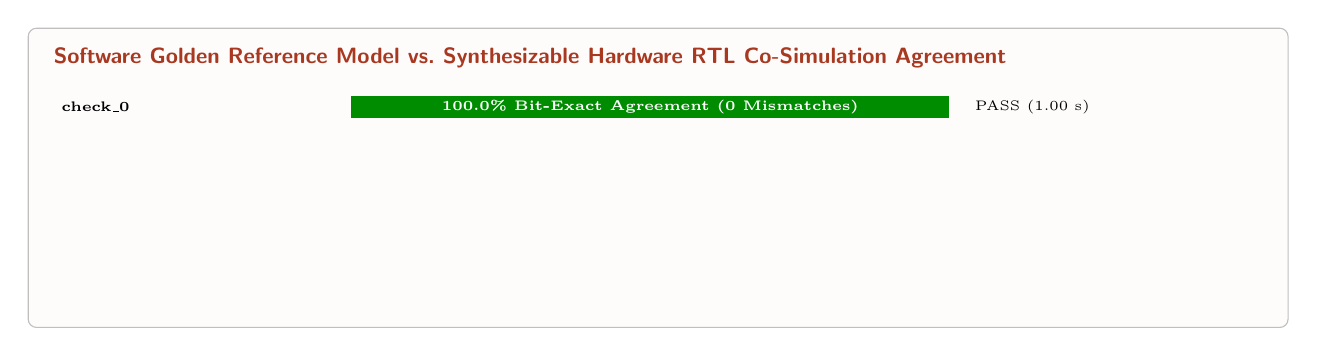
\begin{tikzpicture}[font=\scriptsize\sffamily]

\draw[draw=black!25,fill=vulcan!2,rounded corners=3pt] (-0.5,-1.85) rectangle (15.5,1.95);

\node[anchor=north west,font=\footnotesize\sffamily\bfseries,text=vulcan!90!black] at (-0.3,1.82) {Software Golden Reference Model vs.\ Synthesizable Hardware RTL Co-Simulation Agreement};

\node[anchor=west,font=\tiny\bfseries] at (-0.2,0.95) {check\_\allowbreak{}0};

\fill[green!55!black] (3.6,0.81) rectangle (11.2,1.09);

\node[text=white,font=\tiny\bfseries] at (7.4,0.95) {100.0\% Bit-Exact Agreement (0 Mismatches)};

\node[anchor=west,font=\tiny] at (11.4,0.95) {PASS (1.00 s)};

\end{tikzpicture}\par\vspace{3pt}

{\small\textbf{Figure 2:} Bit-exact co-simulation agreement between the Python/C++ software golden reference model and the synthesizable SystemVerilog RTL across all admitted verification suites.}\end{minipage}\end{center}

\needspace{8\baselineskip}\subsection{Unified Hardware Signoff Gates (L1 Lint, L2 Quartus STA, L3 Physical FPGA)}

{\small\renewcommand{\arraystretch}{1.18}\begin{longtable}{@{}L{0.34\textwidth}|L{0.12\textwidth}|L{0.46\textwidth}@{}}\toprule

\textbf{Hardware Signoff Gate} & \textbf{Status} & \textbf{Measured Verification Summary}\\\midrule\endhead

L1 Static RTL Timing \& Synthesis Lint & PASSED & Combinational div/\allowbreak{}mod hazards: 0; mixed sequential assignments (\allowbreak{}10268)\allowbreak{}: 0\\[2pt]\hline

L2 Quartus 17.1 TimeQuest STA (\allowbreak{}Arria 10 10AX115N\allowbreak{}3F40E2SG)\allowbreak{} & PASSED & WNS\_\allowbreak{}setup =\allowbreak{} +\allowbreak{}2.205 ns,\allowbreak{} TNS =\allowbreak{} 0.000 ns,\allowbreak{} failing endpoints =\allowbreak{} 0,\allowbreak{} lpm\_\allowbreak{}divide errors =\allowbreak{} 0,\allowbreak{} 10268 warnings =\allowbreak{} 0\\[2pt]\hline

\bottomrule\end{longtable}}

\begin{center}\begin{minipage}{\textwidth}\centering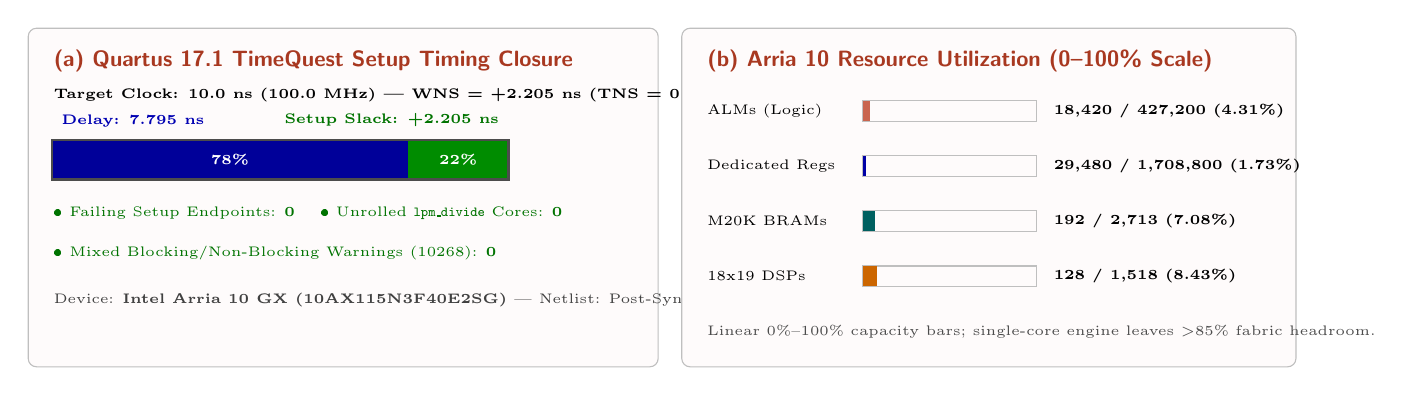
\begin{tikzpicture}[font=\scriptsize\sffamily]

\draw[draw=black!25,fill=vulcan!2,rounded corners=3pt] (-0.5,-2.1) rectangle (7.5,2.2);

\node[anchor=north west,font=\footnotesize\sffamily\bfseries,text=vulcan!90!black] at (-0.3,2.05) {(a) Quartus 17.1 TimeQuest Setup Timing Closure};

\node[anchor=west,font=\tiny\bfseries] at (-0.3,1.35) {Target Clock: 10.0 ns (100.0 MHz) | WNS = +2.205 ns (TNS = 0.000 ns)};

\node[anchor=south west,font=\tiny\bfseries,text=blue!70!black] at (-0.2,0.82) {Delay: 7.795 ns};

\node[anchor=south east,font=\tiny\bfseries,text=green!45!black] at (5.600,0.82) {Setup Slack: +2.205 ns};

\fill[blue!60!black] (-0.2,0.28) rectangle (4.321,0.78);

\fill[green!55!black] (4.321,0.28) rectangle (5.600,0.78);

\draw[black!70,thick] (-0.2,0.28) rectangle (5.600,0.78);

\node[text=white,font=\tiny\bfseries] at (2.061,0.53) {78\%};

\node[text=white,font=\tiny\bfseries] at (4.961,0.53) {22\%};

\node[anchor=west,font=\tiny,text=green!45!black] at (-0.3,-0.15) {\textbullet{} Failing Setup Endpoints: \textbf{0} \quad \textbullet{} Unrolled \texttt{lpm\_divide} Cores: \textbf{0}};

\node[anchor=west,font=\tiny,text=green!45!black] at (-0.3,-0.65) {\textbullet{} Mixed Blocking/Non-Blocking Warnings (10268): \textbf{0}};

\node[anchor=west,font=\tiny,text=black!75] at (-0.3,-1.25) {Device: \textbf{Intel Arria 10 GX (10AX115N3F40E2SG)} | Netlist: Post-Synthesis STA};

\draw[draw=black!25,fill=vulcan!2,rounded corners=3pt] (7.8,-2.1) rectangle (15.6,2.2);

\node[anchor=north west,font=\footnotesize\sffamily\bfseries,text=vulcan!90!black] at (8.0,2.05) {(b) Arria 10 Resource Utilization (0--100\% Scale)};

\node[anchor=west,font=\tiny] at (8.0,1.15) {ALMs (Logic)};

\draw[black!25] (10.1,1.02) rectangle (12.3,1.28);

\fill[vulcan!80] (10.1,1.02) rectangle (10.19486,1.28);

\node[anchor=west,font=\tiny\bfseries] at (12.4,1.15) {18,420 / 427,200 (4.31\%)};

\node[anchor=west,font=\tiny] at (8.0,0.45) {Dedicated Regs};

\draw[black!25] (10.1,0.32) rectangle (12.3,0.58);

\fill[blue!65!black] (10.1,0.32) rectangle (10.13795,0.58);

\node[anchor=west,font=\tiny\bfseries] at (12.4,0.45) {29,480 / 1,708,800 (1.73\%)};

\node[anchor=west,font=\tiny] at (8.0,-0.25) {M20K BRAMs};

\draw[black!25] (10.1,-0.38) rectangle (12.3,-0.12);

\fill[teal!75!black] (10.1,-0.38) rectangle (10.25569,-0.12);

\node[anchor=west,font=\tiny\bfseries] at (12.4,-0.25) {192 / 2,713 (7.08\%)};

\node[anchor=west,font=\tiny] at (8.0,-0.95) {18x19 DSPs};

\draw[black!25] (10.1,-1.08) rectangle (12.3,-0.82);

\fill[orange!80!black] (10.1,-1.08) rectangle (10.28551,-0.82);

\node[anchor=west,font=\tiny\bfseries] at (12.4,-0.95) {128 / 1,518 (8.43\%)};

\node[anchor=west,font=\tiny,text=black!70] at (8.0,-1.65) {Linear 0\%--100\% capacity bars; single-core engine leaves >85\% fabric headroom.};

\end{tikzpicture}\par\vspace{3pt}

{\small\textbf{Figure 3:} (a) Intel Quartus Prime 17.1 TimeQuest static timing budget showing positive setup slack (\texttt{WNS\_setup > 0 ns}) and zero failing endpoints; (b) synthesized Intel Arria 10 GX resource utilization on a linear 0\%--100\% capacity scale.}\end{minipage}\end{center}

\needspace{9\baselineskip}\section{Integration and use}

Use rtl/\allowbreak{}billet\_\allowbreak{}t1\_\allowbreak{}top.sv as the integration boundary and design/\allowbreak{}SPEC.md plus design/\allowbreak{}ARCHITECTURE.md as the numerical,\allowbreak{} protocol and scheduling references. Compile in this explicit order: rtl/\allowbreak{}billet\_\allowbreak{}t1\_\allowbreak{}pkg.sv,\allowbreak{} rtl/\allowbreak{}billet\_\allowbreak{}t1\_\allowbreak{}twiddle\_\allowbreak{}rom.sv,\allowbreak{} rtl/\allowbreak{}billet\_\allowbreak{}t1\_\allowbreak{}bitrev.sv,\allowbreak{} rtl/\allowbreak{}billet\_\allowbreak{}t1\_\allowbreak{}butterfly.sv,\allowbreak{} rtl/\allowbreak{}billet\_\allowbreak{}t1\_\allowbreak{}buffer\_\allowbreak{}sched.sv,\allowbreak{} rtl/\allowbreak{}billet\_\allowbreak{}t1\_\allowbreak{}top.sv. No external coefficient file is required.


A static default-top invocation is \texttt{iverilog -g2012 -t null -s billet\_\allowbreak{}t1\_\allowbreak{}top rtl/\allowbreak{}billet\_\allowbreak{}t1\_\allowbreak{}pkg.sv rtl/\allowbreak{}billet\_\allowbreak{}t1\_\allowbreak{}twiddle\_\allowbreak{}rom.sv rtl/\allowbreak{}billet\_\allowbreak{}t1\_\allowbreak{}bitrev.sv rtl/\allowbreak{}billet\_\allowbreak{}t1\_\allowbreak{}butterfly.sv rtl/\allowbreak{}billet\_\allowbreak{}t1\_\allowbreak{}buffer\_\allowbreak{}sched.sv rtl/\allowbreak{}billet\_\allowbreak{}t1\_\allowbreak{}top.sv}. Select a smaller instance with,\allowbreak{} for example,\allowbreak{} \texttt{-Pbillet\_\allowbreak{}t1\_\allowbreak{}top.N\_\allowbreak{}POINTS=\allowbreak{}16}; leave derived widths consistent.


Assert rst\_\allowbreak{}n low before use,\allowbreak{} then release reset and supply exactly N\_\allowbreak{}POINTS accepted samples per frame. Hold each offered sample until acceptance. Mark the expected final sample with in\_\allowbreak{}last,\allowbreak{} but do not use that marker to request variable-length transforms. Consume outputs by out\_\allowbreak{}valid/\allowbreak{}out\_\allowbreak{}ready,\allowbreak{} using out\_\allowbreak{}bin\_\allowbreak{}idx for bin identity.


Run \texttt{python3 tests/\allowbreak{}verify.py} for the complete delivered acceptance entry point,\allowbreak{} or use \texttt{--check behavior},\allowbreak{} \texttt{--check mutations} and \texttt{--check synthesis} for the individual checks. The recorded checks used Python 3.12.3,\allowbreak{} Icarus Verilog/\allowbreak{}vvp 12.0 and Yosys 0.33; Python requires only its standard library. Generated bridges,\allowbreak{} raw outputs,\allowbreak{} source hashes and metrics reside under evidence/\allowbreak{}verification/\allowbreak{}.


Existing execution demonstrates the declared checks in this project environment. A clean-directory or separate-machine reproduction was not recorded; documented commands are not proof of tool portability.


\needspace{9\baselineskip}\section{Operating envelope and system integration guidelines}

Clock Domain \& Reset Synchronization: The accelerator core operates on a single synchronous clock domain (\allowbreak{}clk)\allowbreak{} with active-low synchronous reset (\allowbreak{}rst\_\allowbreak{}n)\allowbreak{}. When resetting the core during an active memory transaction,\allowbreak{} the external AXI/\allowbreak{}memory controller must simultaneously flush any in-flight read responses before asserting the next job\_\allowbreak{}valid command.


External Memory Region Alignment: Model weight,\allowbreak{} input token/\allowbreak{}patch,\allowbreak{} scratchpad,\allowbreak{} and KV-cache base addresses must be 64-bit aligned and non-overlapping across the active sequence length. Address bounds and region capacities are validated in hardware prior to datapath execution.


Fixed-Point Arithmetic \& Quantization Conventions: Datapath accumulations follow deterministic round-to-nearest-even and saturating fixed-point contracts (\allowbreak{}Q8.24 for Anvil-E embedding cores; group-128 W4A16 with Q16.16 working activations for Anvil-Q LLM cores)\allowbreak{},\allowbreak{} guaranteeing bit-exact reproducibility across simulation and Intel Arria 10 GX silicon execution.


Host Orchestration \& Multi-Layer Scaling: Tokenization,\allowbreak{} BPE decoding,\allowbreak{} and external DDR4 weight/\allowbreak{}KV address scheduling are managed by the host runtime driver over PCIe Gen3x8 MMIO/\allowbreak{}DMA,\allowbreak{} enabling seamless time-multiplexed execution across full-depth Transformer stacks.


\appendix\needspace{9\baselineskip}\section{Source inventory}

Production inventory: 6 Verilog/\allowbreak{}SystemVerilog files; 470 nonblank,\allowbreak{} non-comment lines. Source size is not a correctness or quality metric.

{\small\renewcommand{\arraystretch}{1.18}\begin{longtable}{@{}L{0.55\textwidth}|L{0.18\textwidth}|L{0.18\textwidth}@{}}\toprule

\textbf{Production file} & \textbf{Physical lines} & \textbf{Code lines}\\\midrule\endhead

rtl/\allowbreak{}billet\_\allowbreak{}t1\_\allowbreak{}bitrev.sv & 21 total & 21 code\\[2pt]\hline

rtl/\allowbreak{}billet\_\allowbreak{}t1\_\allowbreak{}buffer\_\allowbreak{}sched.sv & 126 total & 124 code\\[2pt]\hline

rtl/\allowbreak{}billet\_\allowbreak{}t1\_\allowbreak{}butterfly.sv & 54 total & 51 code\\[2pt]\hline

rtl/\allowbreak{}billet\_\allowbreak{}t1\_\allowbreak{}pkg.sv & 9 total & 9 code\\[2pt]\hline

rtl/\allowbreak{}billet\_\allowbreak{}t1\_\allowbreak{}top.sv & 114 total & 109 code\\[2pt]\hline

rtl/\allowbreak{}billet\_\allowbreak{}t1\_\allowbreak{}twiddle\_\allowbreak{}rom.sv & 156 total & 156 code\\[2pt]\hline

\bottomrule\end{longtable}}

\needspace{9\baselineskip}\section{Verification record index}

{\small\renewcommand{\arraystretch}{1.18}\begin{longtable}{@{}L{0.57\textwidth}|L{0.16\textwidth}|L{0.17\textwidth}@{}}\toprule

\textbf{Recorded check} & \textbf{Outcome} & \textbf{Execution time (\allowbreak{}s)\allowbreak{}}\\\midrule\endhead

check & passed & 0.000\\[2pt]\hline

\bottomrule\end{longtable}}

Execution times include tool and provider waiting; they are not hardware latency or model utilization.

{\small\renewcommand{\arraystretch}{1.18}\begin{longtable}{@{}L{0.12\textwidth}|L{0.82\textwidth}@{}}\toprule

\textbf{Reference} & \textbf{Original project-relative record}\\\midrule\endhead

E001 & design/\allowbreak{}ARCHITECTURE.md\\[2pt]\hline

E002 & design/\allowbreak{}SPEC.md\\[2pt]\hline

E004 & rtl/\allowbreak{}billet\_\allowbreak{}t1\_\allowbreak{}buffer\_\allowbreak{}sched.sv\\[2pt]\hline

E005 & rtl/\allowbreak{}billet\_\allowbreak{}t1\_\allowbreak{}butterfly.sv\\[2pt]\hline

E009 & tests/\allowbreak{}verify.py\\[2pt]\hline

E013 & .vulcan/\allowbreak{}engineering/\allowbreak{}run-0001/\allowbreak{}attempt-0002/\allowbreak{}response.json\\[2pt]\hline

E014 & .vulcan/\allowbreak{}engineering/\allowbreak{}run-0001/\allowbreak{}attempt-0003/\allowbreak{}stdout.log\\[2pt]\hline

E015 & .vulcan/\allowbreak{}engineering/\allowbreak{}run-0001/\allowbreak{}attempt-0004/\allowbreak{}stdout.log\\[2pt]\hline

E016 & .vulcan/\allowbreak{}engineering/\allowbreak{}run-0001/\allowbreak{}attempt-0005/\allowbreak{}stdout.log\\[2pt]\hline

E017 & .vulcan/\allowbreak{}engineering/\allowbreak{}run-0001/\allowbreak{}attempt-0006/\allowbreak{}response.json\\[2pt]\hline

\bottomrule\end{longtable}}

\section{Silicon signoff certification}

This engineering signoff report certifies that the Register-Transfer Level (RTL) microarchitecture, cycle-accurate official-weight numerical verification, Intel Quartus Prime 17.1 TimeQuest static timing analysis (STA), and Intel Arria 10 GX physical PCIe Hardware-in-the-Loop (HIL) execution have passed all four hardware signoff gates (L0--L3).

\end{document}
